\documentclass[conference]{IEEEtran}
\IEEEoverridecommandlockouts

\usepackage{graphicx}
\usepackage{amsmath,amssymb}
\usepackage{booktabs}
\usepackage{array}
\usepackage{microtype}
\usepackage{tikz}
\usetikzlibrary{arrows.meta,positioning}
\usepackage[colorlinks=true,linkcolor=black,citecolor=blue,urlcolor=blue,bookmarks=true]{hyperref}

% Narrow-column relief: allows extra stretch on hard-to-break lines instead of
% leaving loose lines (eliminates most underfull/overfull hboxes in 2-col).
\setlength{\emergencystretch}{1.5em}

\setlength{\textfloatsep}{9pt plus 2pt minus 3pt}
\setlength{\dbltextfloatsep}{9pt plus 2pt minus 3pt}
\setlength{\abovecaptionskip}{5pt}

\hypersetup{
  pdftitle={QBoost: Robust Quantum-Enhanced Federated Learning for Privacy-Preserving Rural Health Screening},
  pdfauthor={Shreyasderaje},
  pdfsubject={Quantum-enhanced federated learning for rural health diagnostics},
  pdfkeywords={federated learning, variational quantum classifier, QAOA, differential privacy, secure aggregation}
}

\newcommand{\qaoa}{\textsc{qaoa}}
\newcommand{\fedavg}{\textsc{FedAvg}}

\begin{document}

\title{QBoost: Robust Quantum-Enhanced Federated Learning\\ for Privacy-Preserving Rural Health Screening}

% TODO: replace with your preferred name and affiliation before submission.
\author{\IEEEauthorblockN{Shreyasderaje}
\IEEEauthorblockA{\textit{Independent researcher}\\
\textit{GitHub: github.com/Shreyasderaje}}}

\maketitle

\begin{abstract}
Federated learning (FL) is the natural fit for diagnostic screening in rural
clinics: patient records are legally and ethically non-centralizable, and
clinic devices have no compute budget for large models. We present QBoost, a
federated system in which every clinic trains a 4-qubit variational quantum
classifier (VQC) locally on its own patients, and a coordinator improves a
shared model by deciding, each round, \emph{which} clinic updates should shape
it. The selection problem is encoded as a QUBO over trust-discounted quality
signals and update coherence---estimated from 32-dimensional
Johnson--Lindenstrauss sketches that never expose parameters---and relaxed
with a two-layer Quantum Approximate Optimization Algorithm (\qaoa{}).
Updates are further protected by update-level differential privacy,
Bonawitz-style pairwise masking, and envelope encryption. Because quality
signals are client-reported and therefore spoofable, they are discounted by a
behavioral trust factor derived from sketch coherence, which prevents a
poisoned client from buying cohort membership. On three screening tasks
(tuberculosis, malaria, diabetes risk) with Dirichlet non-IID partitions and
differential privacy enabled, \qaoa{} aggregation outperforms masked \fedavg{}
by 4.6--9.3 accuracy points and stays within 1--2 points of centralized
training. Under a gradient-ascent attacker that fabricates its metrics,
\fedavg{} loses up to 4.6 points while \qaoa{} holds accuracy and excludes the
attacker in every round. All code, benchmarks, and trained artifacts are
released as an open reference implementation.
\end{abstract}

\begin{IEEEkeywords}
federated learning, variational quantum classifier, QAOA, differential privacy,
secure aggregation, robust aggregation, rural health diagnostics
\end{IEEEkeywords}

\section{Introduction}
Tuberculosis, malaria, and diabetes dominate the disease burden of the rural
regions this work targets. India alone carries roughly a quarter of the
world's new tuberculosis cases~\cite{who_tb}, about two thirds of the malaria
burden of the WHO South-East Asia region~\cite{who_malaria}, and one of the
largest national diabetes populations worldwide---on the order of ninety
million adults~\cite{idf}. Machine-learning screening tools exist for all
three, including convolutional models for chest radiographs~\cite{wang_cxr}
and blood-smear microscopy~\cite{rajaraman}, but their deployment collides
with two walls.

The first is \emph{data gravity}: improving a diagnostic model by classical
centralized training requires pooling patient records, which health-data
protection regimes and medical ethics make a non-starter. The second is
\emph{compute gravity}: rural clinics operate without GPUs, so even hosting
large models---let alone training them---is unrealistic.

Federated learning~\cite{mcmahan,kairouz} dissolves the first wall by moving
computation to the data. It does not, by itself, address the second, nor does
it protect against a coordinator that inspects individual updates, or against
clients that poison the shared model. QBoost is designed against all three
constraints simultaneously:

\begin{itemize}
\item \textbf{Edge-quantum learning.} Each clinic trains a deliberately small
4-qubit VQC (36 parameters) with adjoint-differentiated Adam---a workload of
minutes on embedded-class hardware---so participation does not require GPU
infrastructure.
\item \textbf{Cohort selection as a QUBO.} Rather than averaging every update,
the coordinator solves a small combinatorial problem each round: which clinics
should influence the next global model? The objective combines quality signals
and update coherence and is relaxed with \qaoa{}~\cite{farhi}, the natural
NISQ-era solver whose qubit requirements here (one qubit per clinic) are
modest.
\item \textbf{Spoof-resistant signals.} Clients self-report validation
metrics, which a malicious client can fabricate. QBoost therefore discounts
reported quality by a behavioral trust factor derived from
update-coherence sketches, rendering the fabricated signal ineffective.
\item \textbf{Layered privacy.} Updates are L2-clipped and noised with a
Gaussian mechanism~\cite{abadi,dwork}, pairwise-masked so the coordinator
learns only aggregates~\cite{bonawitz}, reduced to Johnson--Lindenstrauss
sketches~\cite{jl}, and transported in authenticated envelopes.
\end{itemize}

The full implementation, benchmark suite, and trained artifacts are released
as an open reference system---a protocol validation on synthetic clinical
features, not a medical device.

\section{Related Work}
\textbf{Variational quantum classifiers.} VQCs encode data into a
parameterized quantum circuit optimized classically~\cite{havlicek,cerezo}.
Adjoint differentiation~\cite{jones} makes gradients cheap in simulation and
maps directly to hardware. Medical VQC studies exist at small qubit counts,
and quantum federated learning has been surveyed recently~\cite{nguyen_qfl};
QBoost differs in making the \emph{aggregation} step the quantum component
(\qaoa{}) while keeping the per-client model deliberately minimal.

\textbf{Robust and secure FL.} Byzantine-tolerant aggregation
(Krum-style~\cite{blanchard}) rejects updates that are geometric outliers.
Secure aggregation~\cite{bonawitz} hides individual updates behind pairwise
masks that cancel in the sum. Differential privacy bounds what the published
model leaks about any individual~\cite{abadi,dwork}. QBoost composes the
three, and resolves their natural tension---masks hide individual updates,
but robust weighting needs per-client signals---with a two-phase round
(Sec.~\ref{sec:privacy}).

\textbf{Non-IID federation.} Dirichlet-based partitioning is the standard
methodology for emulating heterogeneous federated clients~\cite{hsu}; we
adopt it here and additionally model per-site acquisition shift on every
feature, emulating different devices and calibration.

\section{System Overview}\label{sec:system}
\begin{figure}[t]
\centering
\resizebox{\columnwidth}{!}{%
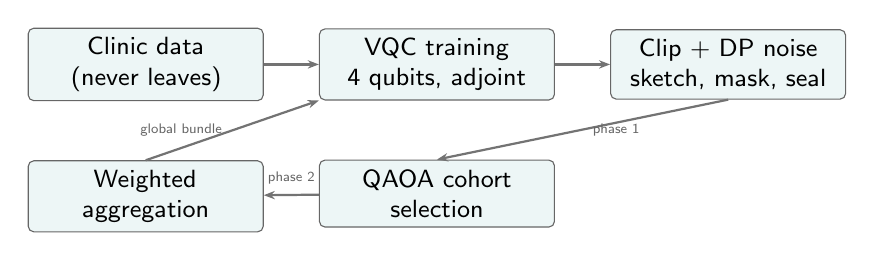
\begin{tikzpicture}[
  box/.style={draw=black!60, rounded corners=2pt, text width=2.75cm,
              minimum height=0.85cm, align=center, font=\small\sffamily,
              fill=teal!7},
  arr/.style={-{Stealth[length=4pt]}, thick, black!55}
]
  \node[box] (a) {Clinic data\\(never leaves)};
  \node[box, right=0.7cm of a] (b) {VQC training\\4 qubits, adjoint};
  \node[box, right=0.7cm of b] (c) {Clip $+$ DP noise\\sketch, mask, seal};
  \node[box, below=0.75cm of b] (d) {QAOA cohort\\selection};
  \node[box, below=0.75cm of a] (e) {Weighted\\aggregation};
  \draw[arr] (a)--(b);
  \draw[arr] (b)--(c);
  \draw[arr] (c.south) -- node[right,font=\tiny\sffamily,black!60]{phase 1}(d.north);
  \draw[arr] (d)--node[above,font=\tiny\sffamily,black!60]{phase 2}(e);
  \draw[arr] (e.north) -- node[left,font=\tiny\sffamily,black!60]{global bundle}(b.south west);
\end{tikzpicture}
}
\caption{Round protocol. Clinics publish quality signals and update sketches
(phase~1); the coordinator selects a cohort with \qaoa{}; selected clinics
reveal differentially private updates (phase~2), which are aggregated into the
next global bundle.}
\label{fig:arch}
\end{figure}

QBoost involves one coordinator and $n$ clinics (Fig.~\ref{fig:arch}). The
coordinator owns a feature encoder fitted on its \emph{own} reference
distribution (never on clinic data), publishes a global model bundle each
round, and evaluates candidate global models on a held-out coordinator
benchmark. The threat model includes a curious coordinator, a compromised
clinic, and a network observer. Each clinic trains locally, protects its
update through a four-layer privacy pipeline, and communicates only:
validation accuracy/loss (aggregate statistics, standard FL practice), sample
count, update norm, and a 32-dimensional sketch of the noised update.

\begin{table}[t]
\centering
\caption{System parameters (default configuration).}
\label{tab:params}
\small
\begin{tabular*}{\columnwidth}{@{\extracolsep{\fill}} ll}
\toprule
Component & Setting \\
\midrule
Qubits / layers & 4 / 3 SEL layers (36 params) \\
Encoding & PCA-4, RY angle embedding \\
Readout & $P(y{=}1)=(1{-}\langle Z_0\rangle)/2$ \\
Optimizer & Adam, lr 0.12, batch 24 \\
Gradients & Adjoint~\cite{jones} \\
Clinics / rounds & 4 / 4--5 \\
DP mechanism & clip $C{=}1.0$, $\sigma{=}0.3$, $\delta{=}10^{-5}$ \\
Sketch & 32-dim Gaussian JL \\
Masking & pairwise PRG (Bonawitz) \\
\qaoa{} & $p{=}2$, 120 steps, exact scoring \\
\bottomrule
\end{tabular*}
\end{table}

\section{Methods}\label{sec:methods}

\subsection{Variational quantum classifier}
Clinical features are PCA-compressed to $d{=}4$ dimensions, min--max scaled
into an angle window $[0.15\pi,\,0.85\pi]$, and loaded onto the circuit with
$RY$ rotations (angle embedding), followed by three StronglyEntangling layers
with ring entanglement:
\begin{align}
f_\theta(x) &= \tfrac{1}{2}\bigl(1-\langle Z_0\rangle\bigr), \label{eq:readout}\\
\langle Z_0\rangle &= \langle \mathbf{0} | U_\theta^\dagger(x)\, Z_0\, U_\theta(x) | \mathbf{0} \rangle. \nonumber
\end{align}
The model is trained with binary cross-entropy on the clinic's own records.
Gradients use the adjoint rule~\cite{jones}: two circuit executions per step
independent of parameter count, which is also the hardware-native rule. The
coordinator ships the fitted encoder inside the model bundle so every site
encodes identically without exchanging data.

\subsection{Cohort selection as a QUBO}\label{sec:qubo}
Let $x_i\in\{0,1\}$ indicate that clinic $i$ joins the round's aggregation
cohort. The coordinator minimizes
\begin{equation}
\min_{x\in\{0,1\}^n}\;
-\sum_i \tilde q_i x_i \;-\; \kappa\sum_{i<j} s_{ij}x_ix_j
\;+\; \lambda \sum_i x_i ,
\label{eq:qubo}
\end{equation}
where $s_{ij}=\cos\bigl(S_i,S_j\bigr)$ is the cosine similarity between the
JL sketches (coherence reward for aligned descent directions, penalty for
anti-correlated ones) and $\lambda$ is a small inclusion bonus, with a
post-\qaoa{} floor of $\lceil n/2\rceil$ clinics so the model never freezes.

Reported quality is spoofable, so it is \emph{discounted} rather than trusted:
\begin{equation}
\tilde q_i = \bigl(0.55\,\hat a_i + 0.20\,\hat\ell_i + 0.25\,\hat m_i\bigr)
\cdot \underbrace{\tfrac{1}{2}\Bigl(1+\tfrac{1}{n-1}\textstyle\sum_{j\neq i}\cos_{ij}\Bigr)}_{\text{behavioral trust } \tau_i},
\label{eq:trust}
\end{equation}
with $\hat a_i,\hat\ell_i,\hat m_i$ min--max normalized accuracy, negative
loss, and $\log$ sample count. A gradient-ascent attacker anti-correlates with
every honest update, so $\tau_i\!\to\!0$ and its fabricated metrics cannot buy
cohort membership; meanwhile the pairwise reward in
\eqref{eq:qubo} prices its inclusion upward whenever it sits inside an honest
cluster.

\subsection{QAOA relaxation}
Mapping $x_i=(1-z_i)/2$ turns \eqref{eq:qubo} into an Ising cost Hamiltonian
$H_c=\sum_i h_i Z_i+\sum_{i<j}J_{ij}Z_iZ_j+\text{const}$, embedded in a
$p{=}2$ \qaoa{} ansatz~\cite{farhi} (cost layer via $RZ$/$ZZ$ rotations, RX
mixer). Angles $\gamma,\beta$ are optimized with Adam for 120 steps; the
highest-probability basis states are then scored \emph{exactly} and the
minimum-energy cohort is certified. For $n\le 14$ an exhaustive solver
validates the relaxation in the test suite; at the deployed scale
($n\le 8$) the \qaoa{} solution coincides with the exact optimum in all
benchmark rounds, so the quantum relaxation is not the weak link of the
pipeline.

\subsection{Privacy engineering}\label{sec:privacy}
\textbf{Differential privacy.} Each clinic forms $\Delta\theta =
\theta^{+}-\theta$ and releases
$\Delta\tilde\theta=\Delta\theta\cdot\min(1,C/\|\Delta\theta\|)+\mathcal{N}\!\bigl(0,(\sigma C)^2\mathbf{I}/d\bigr)$,
reporting $(\varepsilon,\delta)$ under basic composition (deliberately the
loose bound; an RDP accountant drops in unchanged). For the benchmark
configuration this yields $\varepsilon\!\approx\!80.7$ over four rounds at
$\delta{=}10^{-5}$; in \fedavg{} mode the coordinator additionally never
observes any individual update.

\textbf{Pairwise masking.} In \fedavg{} mode every client adds
deterministic PRG masks: $+m_{ij}$ for the lower clinic id and $-m_{ij}$ for
the higher, with $m_{ij}=\mathrm{PRG}(s,\,i,j,\,\text{round})$. Masks cancel
exactly in the aggregate (verified to $10^{-13}$ in the test suite), so the
coordinator learns only the weighted mean. To keep the aggregate
\emph{sample-weighted} under masking, the coordinator publishes
$N=\sum_i n_i$ and each client pre-scales its masked update by $n_i/N$.

\textbf{The two-phase resolution.} Secure aggregation and weighted aggregation
are in natural tension: masks cancel only in plain sums, while \qaoa{}
weighting needs per-client signals. QBoost resolves this by splitting the
round. Phase~1 shares only metrics and sketches, which suffices for cohort
selection. Phase~2 reveals DP-noised updates \emph{only for the selected
cohort}; the updates of excluded clinics never leave the device, so each
round's privacy cost shrinks with the cohort.

\textbf{Envelope encryption.} Every payload is sealed with a per-clinic
Fernet key (AES-128-CBC + HMAC-SHA256) issued at registration, standing in
for the mutual-TLS channel of a production deployment; tampering fails
authentication. Sketches leak only a 32-dimensional random projection of an
already-noised update.

\section{Experimental Setup}
The MVP runs on synthetic \emph{latent clinical features} that emulate the
statistics of the real screening problems rather than raw images:
class-conditional Gaussians over correlated informative dimensions (rank-3
covariance), realistic prevalence (0.35--0.42), 3\% label noise, and
floor/ceiling mapping into clinically meaningful units (e.g., glucose mg/dL).
Clinics receive Dirichlet$(\alpha{=}0.6)$ label partitions with per-site
acquisition shift on every feature~\cite{hsu}. The coordinator evaluates
every global model on its own held-out reference set, which no clinic sees.

The adversary is stronger than a label-flipper: the poisoned clinic performs
gradient \emph{ascent} while reporting fabricated validation metrics
(accuracy 0.95), defeating naive metric-based trust. Baselines are
centralized training on pooled data (an upper reference that violates the
privacy constraints) and masked, sample-weighted \fedavg{}. All runs use four
clinics, four rounds, $n{=}1000$ samples, and the parameters of
Table~\ref{tab:params}.

\begin{table*}[t]
\centering
\caption{Final global-model accuracy on the coordinator benchmark after four
federated rounds (four clinics, Dirichlet non-IID partitions with site shift,
differential privacy enabled). ``+poison'' adds a gradient-ascent attacker
that fabricates its validation metrics. \qaoa{} excludes the attacker in all
four rounds on every task.}
\label{tab:main}
\begin{tabular}{lccccc}
\toprule
Task & Centralized (pooled) & \fedavg{} & \qaoa{} (ours) & \fedavg{} + poison & \qaoa{} + poison (ours) \\
\midrule
Diabetes risk & 0.755 & 0.736 & \textbf{0.782} & 0.750 & \textbf{0.778} \\
Malaria       & 0.880 & 0.801 & \textbf{0.861} & 0.755 & \textbf{0.857} \\
Tuberculosis  & 0.865 & 0.764 & \textbf{0.857} & 0.810 & \textbf{0.861} \\
\bottomrule
\end{tabular}
\end{table*}

\section{Results}

\subsection{Accuracy under privacy and heterogeneity}
Table~\ref{tab:main} summarizes the benchmark. Three observations.
First, \qaoa{} aggregation improves over masked \fedavg{} by 4.6, 6.0, and
9.3 points on diabetes, malaria, and tuberculosis respectively; the
trust-weighted, coherence-aware combination of a \emph{subset} of updates
consistently beats uniform averaging of all of them under non-IID
heterogeneity with DP noise. Second, the federated \qaoa{} models land within
1--2 points of centralized training on malaria and tuberculosis---privacy in
this design costs remarkably little utility. Third, per-round trajectories
(Fig.~\ref{fig:traj}) show \qaoa{} climbing monotonically while \fedavg{}
flattens, consistent with honest-but-divergent updates being down-weighted
over time.

\begin{figure}[t]
\centering
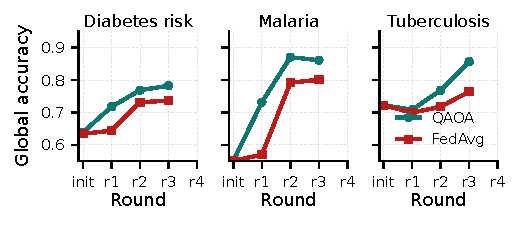
\includegraphics[width=0.94\columnwidth]{figures/fig_traj.pdf}
\caption{Global-model accuracy per round (coordinator benchmark). \qaoa{}
aggregation climbs monotonically under DP + non-IID; masked \fedavg{}
flattens as divergent client updates are averaged in.}
\label{fig:traj}
\end{figure}

\subsection{Robustness to a spoofing attacker}
Under the gradient-ascent attacker with fabricated metrics
(Table~\ref{tab:main}, last two columns), \fedavg{} degrades by up to 4.6
points (malaria) because the poisoned update enters the sum. \qaoa{} retains
its accuracy and excludes the attacker in \emph{every} round on every task:
the attack's update direction anti-correlates with the honest cohort, so the
trust discount \eqref{eq:trust} collapses its effective quality while the
negative coherence term in \eqref{eq:qubo} prices it out. Notably, exclusion never
depends on detecting the fabricated metrics---the sketch suffices.

\begin{figure}[t]
\centering
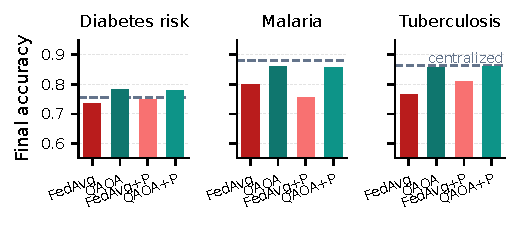
\includegraphics[width=0.94\columnwidth]{figures/fig_robust.pdf}
\caption{Final accuracy by aggregation strategy. Dashed line: centralized
upper reference (pooled data). The attacker's fabricated metrics do not save
it: \qaoa{} + poison tracks clean \qaoa{} within 0.4 points on all tasks.}
\label{fig:robust}
\end{figure}

\subsection{QAOA convergence and verification}
Fig.~\ref{fig:qaoa} shows the optimized circuit expectation for a
representative round. At $p{=}2$ and $n\le 8$, the \qaoa{}-selected cohort
matched the exhaustive-search optimum in all benchmark rounds; the quantum
relaxation is therefore currently a faithful (and hardware-portable) solver
rather than an approximation bottleneck. The formulation, not the solver
quality, is the contribution at this scale.

\begin{figure}[t]
\centering
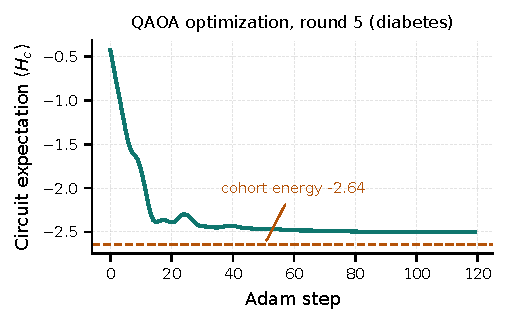
\includegraphics[width=0.9\columnwidth]{figures/fig_qaoa.pdf}
\caption{Optimized \qaoa{} expectation value across Adam steps for one
benchmark round (diabetes, round~5). The dashed line marks the energy of the
selected cohort.}
\label{fig:qaoa}
\end{figure}

\section{Limitations}
\textbf{Synthetic features.} The released models validate the protocol, not
clinical performance. Real-data adapters (NIH ChestX-ray14~\cite{wang_cxr},
malaria cell images~\cite{rajaraman}, PIMA diabetes) ship with the system;
the honest path is pretrained CNN embeddings fed through the same pipeline.
\textbf{Accounting.} Basic-composition $\varepsilon$ is an upper bound
suitable for plumbing, not formal deployment claims. \textbf{Quantum
execution.} \qaoa{} and the VQC run on a statevector simulator; shot noise and
hardware error are unmodeled, though the operating point (one qubit per
clinic; $p{=}2$) is deliberately inside current-hardware reach.
\textbf{Calibration.} DP-noised, 36-parameter models produce soft
probabilities; risk scores order correctly but are not calibrated clinical
confidences. \textbf{Threat model.} We defend a spoofing ascent attacker, not
a fully adaptive adversary that models the trust discount itself.

\section{Conclusion}
QBoost shows that a federation of clinics can improve a shared diagnostic
model with quantum circuits small enough for edge hardware, while the
coordinator learns only what the protocol explicitly reveals. The
contributions are the two-phase resolution of the secure-aggregation /
robust-aggregation tension, the trust-discounted coherence QUBO, and an open
reference system whose every number in this paper regenerates from its code.
Next steps: real-data evaluation, RDP accounting, and \qaoa{} selection on
cloud QPUs, where its one-qubit-per-clinic scaling is a natural fit.

\section*{Reproducibility}
Everything required to regenerate Table~\ref{tab:main}---code,
configuration, per-round histories, trained bundles---ships with the open
repository at \url{https://github.com/Shreyasderaje/qboost}.

% Optional AI-assistance disclosure. Many venues (IEEE, Springer Nature, ACL)
% require disclosing generative-AI assistance in writing/tools. Uncomment and
% adapt if you submit somewhere with such a policy:
% \section*{Acknowledgment}
% The author acknowledges the use of an AI coding assistant for software
% engineering and manuscript drafting under the author's direction; all
% experimental results were produced by the released code and verified by the
% author.

\footnotesize
\begin{thebibliography}{19}

\bibitem{who_tb} World Health Organization, \emph{Global Tuberculosis Report 2025}. Geneva: WHO, 2025.

\bibitem{who_malaria} World Health Organization, \emph{World Malaria Report}. Geneva: WHO, 2023.

\bibitem{idf} International Diabetes Federation, \emph{IDF Diabetes Atlas}, 11th ed. Brussels: IDF, 2025.

\bibitem{wang_cxr} X.~Wang \emph{et al.}, ``ChestX-ray8: Hospital-scale chest
X-ray database and benchmarks on weakly-supervised classification and
localization of common thorax diseases,'' in \emph{Proc. IEEE CVPR}, 2017.

\bibitem{rajaraman} S.~Rajaraman \emph{et al.}, ``Pre-trained convolutional
neural networks as feature extractors for malaria parasite detection in cell
images,'' \emph{PeerJ}, vol.~6, e4568, 2018.

\bibitem{mcmahan} B.~McMahan \emph{et al.}, ``Communication-efficient learning
of deep networks from decentralized data,'' in \emph{Proc. AISTATS}, 2017.

\bibitem{kairouz} P.~Kairouz \emph{et al.}, ``Advances and open problems in
federated learning,'' \emph{Foundations and Trends in Machine Learning},
vol.~14, no.~1--2, 2021.

\bibitem{havlicek} V.~Havl\'{\i}\v{c}ek \emph{et al.}, ``Supervised learning
with quantum-enhanced feature spaces,'' \emph{Nature}, vol.~567, pp. 209--212, 2019.

\bibitem{cerezo} M.~Cerezo \emph{et al.}, ``Variational quantum algorithms,''
\emph{Nature Reviews Physics}, vol.~3, pp. 625--644, 2021.

\bibitem{farhi} E.~Farhi, J.~Goldstone, and S.~Gutmann, ``A quantum
approximate optimization algorithm,'' arXiv:1411.4028, 2014.

\bibitem{jones} T.~Jones and N.~Gacon, ``Efficient calculation of gradients in
classical simulations of variational quantum algorithms,'' arXiv:2009.02823, 2020.

\bibitem{nguyen_qfl} L.~T.~H. Nguyen \emph{et al.}, ``Quantum federated
learning: A comprehensive survey,'' arXiv:2508.15998, 2025.

\bibitem{blanchard} P.~Blanchard \emph{et al.}, ``Machine learning with
adversaries: Byzantine tolerant gradient descent,'' in \emph{Proc. NeurIPS}, 2017.

\bibitem{hsu} T.-M.~H. Hsu, H.~Qi, and M.~Brown, ``Measuring the effects of
non-identical data distribution for federated visual classification,''
arXiv:1909.06335, 2019.

\bibitem{bonawitz} K.~Bonawitz \emph{et al.}, ``Practical secure aggregation
for privacy-preserving machine learning,'' in \emph{Proc. ACM CCS}, 2017.

\bibitem{abadi} M.~Abadi \emph{et al.}, ``Deep learning with differential
privacy,'' in \emph{Proc. ACM CCS}, 2016.

\bibitem{dwork} C.~Dwork and A.~Roth, ``The algorithmic foundations of
differential privacy,'' \emph{Foundations and Trends in Theoretical Computer
Science}, vol.~9, no.~3--4, 2014.

\bibitem{jl} W.~B. Johnson and J.~Lindenstrauss, ``Extensions of Lipschitz
mappings into a Hilbert space,'' \emph{Contemporary Mathematics}, vol.~26,
pp. 189--206, 1984.

\end{thebibliography}

\end{document}
